%! TEX root = ../listas_completas.tex
\section{Lista 2}
\subsection{Questão 1}
Uma barra de torção da suspensão traseira do fusca, possui um comprimento de
\SI{40}{cm} e o diâmetro de \SI{40}{mm}, sendo feita de ferro fundido dúctil.
Tendo o veículo 800 kg e considerando que seu peso se distribua igualmente nas 4
rodas, determine sua rigidez elástica da barra de torção.

\resol
Dados: $m=800\kg$; $l = \SI{40}{cm}$; $d = \SI{40}{mm}$;

material: ferro fundido dúctil;

$ E=\SI{168,9}{\giga\pascal}$; $G =\SI{9,4}{\giga\pascal}$;
$ \rho =\SI{6,9}{Mg\per{m^3}} $

Eixo oco:
\[ k_{eq} = \frac{\pi\, G\times (D^4-d^4)}{32\,L} \]

Eixo simples:
\[
    k_{eq} = \frac{\pi\cdot G\cdot (D^4)}{32\,L}=
\]
\[
=\frac{\pi\cdot 9,4 \cdot (40\times 10^{-3})^{4} }{32\cdot
0,04}=\SI{5906,2}{\newton\per\meter}
\]
\subsection{Questão 2}
Uma viga mono engastada de seção transversal uniforme, suporta uma carga
estática de 200kg, aplicada na extremidade B, sofrendo uma deflexão $\delta$.
Sabendo que L = 3,5 m, feita em aço carbono com
perfil quadrado de \SI{3}{mm} de lado, determine:
\begin{enumerate}[label=\alph*)]
    \item constante elástica de mola equivalente da viga
    \item após a colocação de uma mola na extremidade da viga a deformação
        reduziu 25\%, qual a constante elástica desta mola instalada?
\end{enumerate}

\begin{figure}[ht]
    \centering
    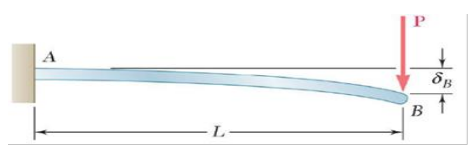
\includegraphics[width=0.4\textwidth]{imagens/lista_2_questao_2.png}
\end{figure}

\resol

Dados: viga mono engastada $m=200 \kg$ $L=3,5 \mathrm{m}$, aço carbono, perfil
quadrado $a=3 \mm$; $E=\SI{206,8}{\giga\pascal}$;  $G=\SI{11,7}{\giga\pascal}$
\[
    I=\frac{a^4}{12} = \frac{(3\times 10^{-3})^4}{12}=\SI{6,75d-12}{m^4}
\]
\textbf{item a --} Antes de colocar a mola.
Substituindo dados na equação:
\[
k_{eq}=\frac{3\, E I}{L^3}=\SI{0,098}{N /m}
\]
\textbf{item b --} Após colocação da mola.
$W=200\kg \times 9,81 = 1962\mathrm{N}$
\[
    \delta_{sis}=0,75\delta_{0}=0,75 \frac{W L^3}{3E I}
\]
Substituindo os dados, a deformação do sistema fica:
\[
    \delta_{sis}=15065,7\mathrm{m}
\]
Sabendo que $W=k_{eq}\times \delta$,
\[
    k_{eq}=\frac{1962}{15065,7}=\SI{0,13}{\newton\per\meter}
\]

\subsection{Questão 3}
Um eixo da hélice de propulsão de um navio, é feito de aço carbono oco, o qual
possui o diâmetro interno de \SI{10}{cm} e o externo de \SI{25}{cm} e
comprimento de \SI{2}{m}.
\begin{enumalpha}
    \item Determine a rigidez equivalente deste eixo.
    \item Devido a constantes problemas de corrosão, o mesmo foi substituído por
um eixo de aço inox, sendo que na parte oca, foi introduzido um material feito
de ferro fundido cinzento. Analisando somente com
relação à rigidez elástica. O novo eixo é equivalente ao original? Justifique.
\end{enumalpha}

\resol

\textbf{item a --} O eixo é oco e sob torção:
\begin{equation}\label{eq:rigidez_eixo_oco}
k_t=\frac{\pi\,G \left( D^{4}-d^{4} \right)  }{32L}
\end{equation}
Substituindo os dados na equação, obtemos:
\[
k_t=\SI{2,18d6}{\newton\per\meter}
\]
\textbf{item b --} A fazer.

\subsection{Questão 4}
Uma viga de ferro fundido cinzento, é montada em balanço em uma máquina, e
suporta uma carga de 45 kg. Para reduzir sua deformação foi montado dois apoios
de molas em sua extremidade, conforme ilustrado na figura abaixo. Tendo as molas
rigidez de \SI{150}{\newton\per\meter} cada, e o comprimento da viga é de
\SI{150}{cm}, sendo esta um perfil circular de diâmetro igual a \SI{10}{cm}.
Determine:

a) A rigidez do sistema de sustentação do equipamento.
b) Qual a flexão do sistema em mm.

\resol

\textbf{item a --} Rigidez do sistema:
(associação em paralelo)
\[
    k_{eq_{mola}}=k_1+k_2=\SI{300}{\newton\per\meter}
\]
\[
    k_{eq_{barra}}=\frac{3E I}{L^3}
\]

A rigidez equivalente do sistema será:

$k_{eq_{sis}} =k_{eq_{mola}} + k_{eq_{barra}}$
\[
    k_{eq_{sis}}=451,58\mathrm{kN/m}
\]

\textbf{item b --} A deformação será:

$W=k\delta$
\[
    \delta=\frac{W}{k}=\frac{\SI{441,45}{\newton}}{\SI{451,58d
    3}{\newton\per\meter}}=0,98\mm
\]

\subsection{Questão 5}
Um guindaste de construção civil, trabalha com um sistema de 2 cabos de
aço-carbono para elevação de carga, considerando que ele pode atuar com altura
máxima de \SI{30}{m} e tendo os cabos o diâmetro de \SI{20}{mm} , sendo o
guindaste capaz de elevar até 1 tonelada, considere o caso extremo e responda:
Determine a rigidez elástica do sistema.

\resol
A carga atuante é dada por:

$W = \SI{1000}{kg}\times \SI{9,81}{m /s^2} = \SI{9810}{N}$

Situação extrema: $L = \SI{30}{m}$

Momento de inércia:
\[
    I = \frac{\pi \cdot 20^{4}}{64}= \SI{7853,98}{mm^4}
\]
Cabo sob carregamento axial. Referência: RAO pg 14:
\[
    k_r=\frac{A E}{L}=\frac{\pi d^{2}E}{4L} = \frac{\pi (20\times 10^{-3})^2 \cdot 206,8 \times 10^9 }{4\cdot 30}
\]
$k_{r}=\SI{2,16}{MN /m}$

Como são dois cabos associados em paralelo, temos:

$k_{eq}= 2\times k_{r}= \SI{4,32}{\mega\newton\per\meter}$

\subsection{Questão 6}%
Duas viga de ferro fundido cinzento, é montada em balanço, sobre elas é montado
um condensador de ar condicionado, cuja massa é de \SI{25}{kg}. Sendo o
comprimento da viga é de \SI{50}{cm}, tendo esta um perfil quadrado de aresta
igual a \SI{2}{cm}. Considere que a carga esteja aplicada na extremidade da
viga. Determine a flexão sofrida por cada viga em mm.

\resol
$W=25\times 9,81 = \SI{245,25}{N}$

$E=\SI{103,4}{GPa}$; $I=\frac{a^4}{12}=\SI{13,33d-9}{m^4}$

\[ k_{eq}=\frac{3E I}{L^3}=\frac{3\cdot 103,4\times 10^{9} \cdot 13,33 \times 10^{-9}}{0,5} \]
\[
k_{eq} = \SI{8269,9}{N /m}
\]

$\delta = \frac{W}{k}$; como são duas vigas, a carga $W$ é dividida.
\[
\delta = \frac{245,25}{2\cdot 8269,9} = \SI{0,0148}{m} = \SI{14,8}{mm}
\]
